\chapter{Extras to remove later}

Some useful commands that were in the template

Texte en \emph{italique}, \textsc{petites majuscules}, mot \mbox{insécable}.\\
Texte \ul{souligné}, \hl{surligné}, \textbf{gras}.\\
Texte entre ``guillemets''.\\
Police \texttt{monospace}.\\
Un mot courant en réseautique mobile: n\oe{}ud\footnote{Note de bas de page.}.\\
L'objet RSVP \texttt{SENDER\_TEMPLATE}.\\
%Nom d'un auteur: \citeauthor{RFC_IPv4}.\\
Une architecture 32~bits.\\
%%
%%  CONCEPTS DE BASE / BASIC CONCEPTS
%%
\section{Définitions et concepts de base}  % environ 2-3 pages

\david{Write about all these base concepts}
\begin{itemize}
    \item Tree
    \item Graph
    \item \acs{DFS}
    \item molecules? maybe? as in a graph of atoms
\end{itemize}




\begin{flushleft}
1\iere{} utilisation d'un acronyme: \gls{cp}.\\
2\ieme{} utilisation d'un acronyme: \gls{cp}.\\
Acronyme au long: \acrlong{cp}.\\
\end{flushleft}

\subsection{Une sous-section}
Un URL: \href{http://www.polymtl.ca}{École Polytechnique de Montréal}.

\subsubsection{Une sous-sous-section}
Les besoins des flots de données peuvent être catégorisés selon
quatre paramètres importants \cite{Fraas2010} ou:
\begin{itemize}
\item la fiabilité (acheminement des données avec succès)~;
\item le délai de \mbox{bout-en-bout} de la source vers la destination~;
\item la variation du délai de \mbox{bout-en-bout} (\emph{jitter})~;
\item la bande passante requise (le débit des informations).
\end{itemize}

\paragraph{Le niveau paragraphe} est plus bas encore dans la hiérarchie\ldots
Une citation entre parenthèses \cite{Chen2009}.
ou des citations entre parenthèses \cite{Haist2014,Senjian2015,Madani2010}.

\clearpage

%%
%% ELEMENTS DE LA PROBLEMATIQUE
%%
\section{Éléments de la problématique}  % environ 3 pages
La description de \mbox{l'en-tête} commun de RSVP est détaillée ci-dessous:\\
\begin{tabular}{p{1in}p{4.5in}}
&\\ % Ligne vide
\texttt{Ver}: & \texttt{4 bits}\\
          & Version du protocole. La version actuelle est~1.\\[5pt]
\texttt{Flags}: & \texttt{4 bits}\\
          & Aucun Flag n'est défini. L'émetteur doit (\textbf{MUST})
          mettre le champ à zéro et le récepteur doit (\textbf{MUST})
          ignorer ce champ.\\[5pt]
\texttt{Msg Type}: & \texttt{8 bits}\\
          & Type de message\\[5pt]
\texttt{Checksum}: & \texttt{16 bits}\\
          & Complément à un du complément à un de la somme des champs
          de \mbox{l'en-tête}, avec le champ Checksum à~0 pour des
          fins de calcul. La valeur~0 signifie qu'aucun Checksum n'a
          été transmis. Si le résultat du calcul du Checksum donne~0,
          la valeur 0xFFFF doit être stockée dans ce champ.\\[5pt]
\texttt{TTL}: & \texttt{8 bits}\\
          & Valeur originelle du champ \texttt{TTL} utilisée pour
          transmettre ce message.\\[5pt]
\texttt{Reserved}: & \texttt{8 bits}\\
          & Réservé pour usage futur. L'émetteur doit (\textbf{MUST})
          mettre le champ à zéro et le récepteur doit (\textbf{MUST})
          ignorer ce champ.\\[5pt]
\texttt{Length}: & \texttt{16 bits}\\
          & Longueur totale du message en octets, incluant
          \mbox{l'en-tête} commun et tous les objets de longueur
          variable.
\end{tabular}

\subsection{Autres types de structures de données}
L'énumération:
\begin{enumerate}
\item Un item~;
\item Un autre item.
\end{enumerate}


\subsection{Le protocole IPv6}
Voir la Figure~\ref{fig:IPv6} pour plus de détails. Le champs DSCP est
décrit dans le Tableau~\ref{tab:RangesDSCP}.

\begin{figure}[htb]
% [htb] place la figure ici + en haut ou en bas de la page. 
% [htb] places the figure here + top or bottom of the page. 
% Vous pouvez également utiliser [tb] pour placer les figures en haut ou en bas de la page et [p] pour les placer sur une page ne contenant que des flottants (ex. : tableaux, figures).
% You can also use [tb] for placing figures on the top or the bottom of a page and [p] for a figure placed on a page containing only floats (ex.: tables, figures).
% Plus d'informations / More information here: https://www.ctan.org/tex-archive/info/epslatex/english 
\centering
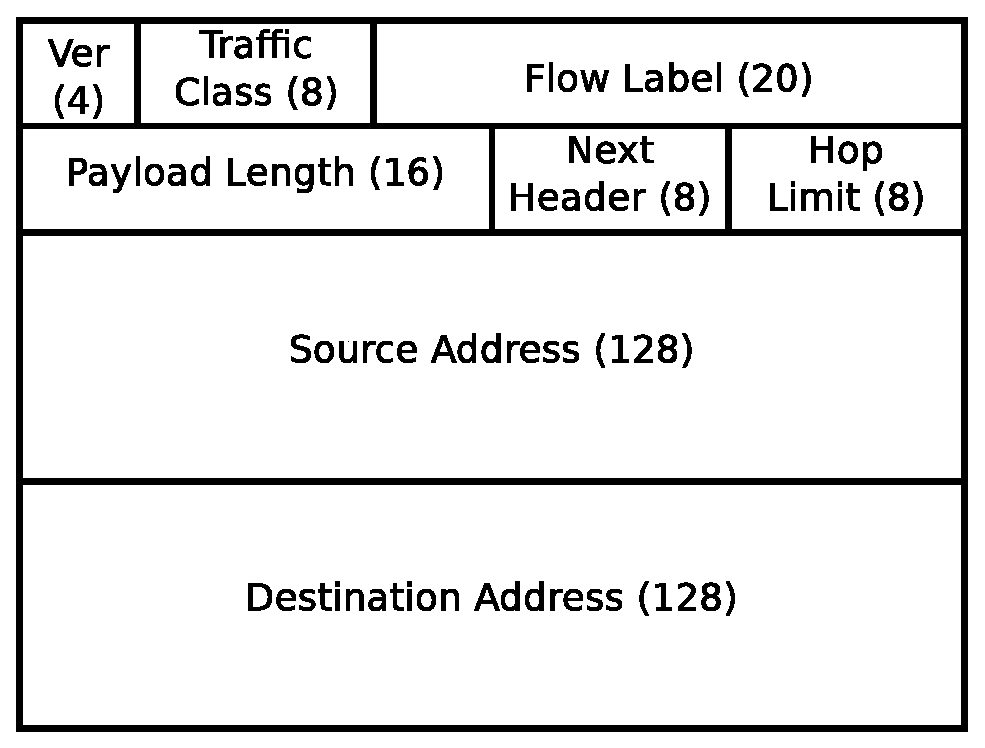
\includegraphics[width=4in]{IPv6_header}
\caption{L'en-tête IPv6}
\label{fig:IPv6}
\end{figure}

\begin{table}[htb]
\caption{Plages de valeurs pour le champ \texttt{DSCP}}
\centering
\begin{tabular}{|c|c|l|}
\hline\rowcolor[gray]{0.8}\color{black}
Plage & Valeurs & Règle d'assignation\\\hline
1 & xxxxx0 & Assignation par une norme de l'IANA\\\hline
2 & xxxx11 & Expérimentation/Usage local\\\hline
3 & xxxx01 & Expérimentation/Usage local (pourrait être jointe à la plage 1)\\\hline
\end{tabular}
\label{tab:RangesDSCP}
\end{table}

% On veut éviter que la figure et le tableau soient placés au-delà de la section courante.
% To prevent the figure and table from being positioned outside of the current section. 
\FloatBarrier


%%
%% OBJECTIFS DE RECHERCHE / RESEARCH OBJECTIVES
%%
\section{Objectifs de recherche}  % 0.5 page
Les objectifs de la recherche sont de concevoir un algorithme $O(n)$.


%%
%% PLAN DU MEMOIRE / THESIS OUTLINE
%%
\section{Plan du mémoire}  % 0.5 page

Voir la Figure~\ref{fig:Layers} pour plus de détails. 

\begin{figure}[htb]
\centering
\includegraphics[width=4in]{demo_tikz}
\caption{Couches}
\label{fig:Layers}
\end{figure}


Un tableau : / A table:
\begin{table}[htb]
  \centering
  \caption{Constantes et variables du modèle analytique}
  \begin{tabular}{|c|l|}
    \hline\rowcolor[gray]{0.8}\color{black}
    Symbole         & Description\\\hline
    $\lambda$       & Taux d'arrivée moyen des requêtes de réservation de ressources\\\hline
    $\frac{1}{\mu}$ & Durée moyenne d'une session\\\hline
    $C$             & Capacité d'une cellule (nombre de sessions supportées)\\\hline
    $v_{moy}$       & Vitesse moyenne des MN dans le réseau d'accès\\\hline
    $L$             & Longueur d'un côté d'une cellule carrée\\\hline
    $n$             & Nombre moyen de MN dans une cellule\\\hline
    $\rho$          & Charge d'une cellule\\\hline
    $P_b$           & Probabilité de blocage d'une requête de réservation\\\hline
    $P_f$           & Probabilité d'interruption forcée d'une session\\\hline
    $P_c$           & Probabilité de compléter une session avec succès\\\hline
    $\Delta{}T$     & Délai de transmission\\\hline
  \end{tabular}
  \label{tab:Definitions}
\end{table}

La formule d'\mbox{Erlang-B}:
\begin{equation}
  P_b = \frac{\frac{\rho^C}{C!}}{\sum\limits_{x=0}^{C}\frac{\rho^x}{x!}}
  \label{eq:Pblock}
\end{equation}

Une autre équation : / Another equation:
\begin{equation}
  \begin{split}
    P_c &= (1 - P_b) \times (1 -  P_f)^N\\
        &= (1 - P_b)^{N+1}
  \end{split}
  \label{eq:ProbComplete}
\end{equation}

Enfin, l'expression suivante indique le moment à partir duquel les
réservations de ressources sont en place:
\begin{equation}
  \Delta{}T_{init} =
  \begin{cases}
    2\Delta{}T_{E2E} & \Delta{}T_{wan} > (\Delta{}T_{rad} + \Delta{}T_{net})\\
    \Delta{}T_{E2E} + 3(\Delta{}T_{rad} + \Delta{}T_{net}) & \text{sinon}
  \end{cases}
  \label{eq:InitCost}
\end{equation}

\paragraph{Le taux de paquets perdus} correspond au nombre de paquets
éliminés à cause d'une erreur de \emph{checksum} à un n\oe{}ud
quelconque ou d'une situation de congestion. Le taux de paquets perdus
pour un chemin est déterminé de la façon suivante:
\begin{equation}
  \label{eq:genPLR}
  PLR_P = 1 - \prod_{i=1}^N(1 - PLR_i)
\end{equation}

Toutefois, si les taux d'erreurs sont très faibles, comme c'est
généralement le cas pour des liens optiques, on peut approximer
$PLR_P$ de façon à le transformer en un paramètre additif:
\begin{equation}
  \label{eq:approxPLR}
  \begin{split}
    PLR_{L_1 \oplus L_2} &= 1 - (1 - PLR_1)(1 - PLR_2)\\
    &= 1 - (1 - PLR_2 - PLR_1 + \underbrace{PLR_1
      \times PLR_2}_\text{négligeable})\qquad PLR_1 \ll 1,
    PLR_2 \ll 1\\
    &\approx PLR_1 + PLR_2
  \end{split}
\end{equation}

\clearpage

Une courbe : / A curve:
\begin{figure}[htb]
\centering
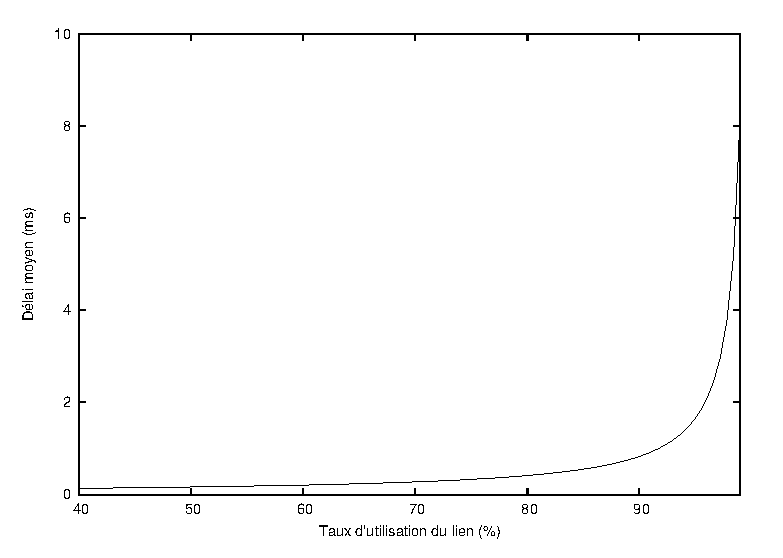
\includegraphics[width=5in]{LinkUsage}
\caption{Délai moyen en fonction du taux d'utilisation d'un lien}
\label{fig:LinkUse}
\end{figure}

\selectlanguage{english}
This paragraph is formatted by \LaTeX{} according to the standard rules of the
English language (\mbox{e.g.} hyphenation).
\selectlanguage{french}

L'arithmétique en virgule flottante peut entraîner des erreurs
d'approximation et il est important d'en être conscient
\cite{Rossi2011}.

De même, les calculs effectués sur une carte graphique (GPU) peuvent
introduire des erreurs d'approximation \cite{DeSantis2002, Cohen2006,
  Thorsson2014, Schirmer2012, Sakai2015, Electrical2006,
  Min2016, Massicotte2013, Kaliouby1987, Daintith2010, Haist2014, Kizza2013,
  Manasreh2011, Brydson1999, Boyce2002}.




Lorem ipsum dolor sit amet, non faucibus ut, ante integer tristique odio
vitae turpis in. Euismod ullamcorper urna eget sollicitudin consectetuer,
dolor a. Ridiculus volutpat fusce, montes ipsum placerat, eu malesuada
maecenas a odio per, est pellentesque integer auctor sed ut sed, lectus
sodales orci ornare. Donec neque turpis vehicula. Duis vel sapien nec massa
lobortis nonummy. Feugiat ultrices urna mauris \cite{Boyer2006}.

Potenti erat molestie ridiculus placerat, viverra ut felis porttitor,
rhoncus accumsan non, dui magna quam justo, ultrices massa ut phasellus
donec viverra mauris \cite{Choy2023a}. Mauris a, dictumst risus a ornare velit nulla
ultricies, neque leo pellentesque, sit sed et suscipit excepteur
aenean. Venenatis sodales, odio nostra in id nobis scelerisque, venenatis
sociosqu gravida blandit orci pellentesque, tincidunt velit sed elementum
lacus pretium nunc, aenean vel dui id \cite{Corrosion2018}. Elit placerat id dui nunc mollis,
diam sapien porta, ipsam elit magna imperdiet amet, erat feugiat, et eros
morbi feugiat velit fringilla. Lacinia phasellus lacinia magna nunc sed, a
rhoncus, sem eget, dui aliquam sit sed leo beatae non, quisque justo
dignissim \cite{Choy2023b,Choy2023}.

Torquent curabitur magnis nullam viverra scelerisque, per lacus pellentesque
vivamus, mauris aliquam sem lacus vivamus nullam porta \cite{IEEE2023}. Vivamus donec
maecenas nunc orci massa, orci neque luctus leo non, mauris quis metus
sagittis. Voluptatibus gravida interdum. Magna duis nulla odio lacus fugiat
non. Magna fusce nunc, eget pellentesque nec. Imperdiet non magna
sollicitudin pellentesque, fusce erat interdum diam tellus vel, vitae
iaculis lectus varius suspendisse. Ac vel a in semper tellus, lobortis sed,
ipsum volutpat. Mauris a nunc aliquam metus nec, eu et id risus, diam
integer molestie suspendisse, sed wisi. Metus sed justo sodales sapien
molestie, suspendisse sem viverra ac proin, lorem luctus at tellus, velit mi
morbi orci in vestibulum, dignissim urna ornare id donec. Suspendisse non
enim euismod odio elit mauris, consectetuer pellentesque faucibus velit ante
lacinia sed \cite{Gervais2013}.

Et dui erat. Wisi lorem eleifend cursus do donec, sed vel fermentum nec, a a
in pharetra \cite{Ledevoir2013}. Ultricies risus, eget habitasse in, consectetuer metus in
auctor ac pellentesque curabitur, pulvinar aliquet eget. Mattis eget
venenatis dolor, nunc sem sed massa, urna scelerisque a magnis, neque elit
nec aliquam nonummy ac accusantium. Id vivamus nunc, erat justo tellus,
scelerisque habitasse accumsan tellus, pede sem vestibulum velit in et
eleifend. Nulla massa aenean integer dui. Suscipit nunc purus, rutrum velit,
mi torquent elementum in tincidunt. Maecenas nulla integer fringilla dapibus
tellus sit, enim amet magna eu erat, libero consectetuer nisl sapien, in
ultricies neque arcu sodales sagittis \cite{Electrical2023}.

Lorem ipsum dolor sit amet, non faucibus ut, ante integer tristique odio
vitae turpis in. Euismod ullamcorper urna eget sollicitudin consectetuer,
dolor a. Ridiculus volutpat fusce, montes ipsum placerat, eu malesuada
maecenas a odio per, est pellentesque integer auctor sed ut sed, lectus
sodales orci ornare. Donec neque turpis vehicula. Duis vel sapien nec massa
lobortis nonummy. Feugiat ultrices urna mauris \cite{Gazette2017}.

Potenti erat molestie ridiculus placerat, viverra ut felis porttitor,
rhoncus accumsan non, dui magna quam justo, ultrices massa ut phasellus
donec viverra mauris. Mauris a, dictumst risus a ornare velit nulla
ultricies, neque leo pellentesque, sit sed et suscipit excepteur
aenean. Venenatis sodales, odio nostra in id nobis scelerisque, venenatis
sociosqu gravida blandit orci pellentesque, tincidunt velit sed elementum
lacus pretium nunc, aenean vel dui id. Elit placerat id dui nunc mollis,
diam sapien porta, ipsam elit magna imperdiet amet, erat feugiat, et eros
morbi feugiat velit fringilla. Lacinia phasellus lacinia magna nunc sed, a
rhoncus, sem eget, dui aliquam sit sed leo beatae non, quisque justo
dignissim \cite{Anschutz2011}.

Torquent curabitur magnis nullam viverra scelerisque, per lacus pellentesque
vivamus, mauris aliquam sem lacus vivamus nullam porta. Vivamus donec
maecenas nunc orci massa, orci neque luctus leo non, mauris quis metus
sagittis. Voluptatibus gravida interdum. Magna duis nulla odio lacus fugiat
non. Magna fusce nunc, eget pellentesque nec. Imperdiet non magna
sollicitudin pellentesque, fusce erat interdum diam tellus vel, vitae
iaculis lectus varius suspendisse \cite{Druide2023}. Ac vel a in semper tellus, lobortis sed,
ipsum volutpat. Mauris a nunc aliquam metus nec, eu et id risus, diam
integer molestie suspendisse, sed wisi. Metus sed justo sodales sapien
molestie, suspendisse sem viverra ac proin, lorem luctus at tellus, velit mi
morbi orci in vestibulum, dignissim urna ornare id donec. Suspendisse non
enim euismod odio elit mauris, consectetuer pellentesque faucibus velit ante
lacinia sed \cite{Guttag2011, Com2018, Audevart2018}.

Et dui erat. Wisi lorem eleifend cursus do donec, sed vel fermentum nec, a a
in pharetra \cite{Gouvernement2023}. Ultricies risus, eget habitasse in, consectetuer metus in
auctor ac pellentesque curabitur, pulvinar aliquet eget \cite{Hinton2016}. Mattis eget
venenatis dolor, nunc sem sed massa, urna scelerisque a magnis, neque elit
nec aliquam nonummy ac accusantium \cite{Corrosion2018}. Id vivamus nunc, erat justo tellus,
scelerisque habitasse accumsan tellus, pede sem vestibulum velit in et
eleifend. Nulla massa aenean integer dui. Suscipit nunc purus, rutrum velit,
mi torquent elementum in tincidunt. Maecenas nulla integer fringilla dapibus
tellus sit, enim amet magna eu erat, libero consectetuer nisl sapien, in
ultricies neque arcu sodales sagittis \cite{CSA2002}.